\ifdefined\included
\else
\setcounter{chapter}{2} %% Numéro du chapitre précédent ;)
\dominitoc
\faketableofcontents
\fi

\chapter{Ontologenius: A long-term semantic memory}
\chaptermark{Ontologenius}
\label{chap:ontologenius}
\minitoc

In this chapter, we present the software Ontologenius. It is a lightweight and open-source software to store ontology, perform reasoning on, update it, and query it. At the difference of other software, Ontologenius has been developed especially for \acrlong{hri} application. In this way, it is able to manage several ontology instances in parallel and put a focus on the concepts' names in natural language. It aims to be used as a server, common to an entire robotic architecture, providing consistent and always up to date knowledge to any other component of the architecture. Consequently, it is thread-safe and can be queried by several components at a time while being constantly updated.

An earlier stage of this contribution had been presented and publish at the RO-MAN 2019 conference~\cite{sarthou_2019_ontologenius}. Due to the evolution of the software since this publication, the current chapter presents new features and a more mature contribution.

\section{Design and features}

In this section, we first explain our choice to use ontology as a means of representing knowledge, both from the point of view of its expressiveness and its growing use in robotics. Then, we present the wanted features for software managing such an ontology and the level of expressiveness we have selected for this software. Finally, we draw a formalism of the kind of ontology we use all along this thesis.

\subsection{Why an ontology?}

In cognitive psychology, we saw that semantic memory refers to the encyclopedic knowledge of words associated with their meanings. After several studies, by studying, among other things, participant response times to questions, some authors have proposed a model of this semantic memory as being a semantic network~\cite{collins_1969_retrieval, collins_1970_does}. With this model, they put the hypothesis that knowledge is organized in a hierarchic way, respecting a principle of inclusion among classes. For example, a class representing the concept of cat would inherit an upper class, representing the concept of animal. In addition, instances of these classes would be linked to others through properties, and in the same way, as for the classes, a notion of hierarchy over the properties would exist. Such a structure of knowledge in humans would allow a cognitive economy as well as efficient storage of this knowledge. Even if not the first to formalize the principle of a semantic network, Collins and Quillian have provided prominent works and computer implementations.


As reported in~\cite{prasad_2020_knowledge}, such a semantic network, also call semantic graph or knowledge graph, is today frequently used as knowledge representation in robotic application to represent among others:

\begin{itemize}
  \item the categories of entities at diffrent level of abstraction~\cite{balint_2018_variations}, like a handle is a physical object
  \item the carateristics of entities~\cite{tenorth_2017_representations}, like a fidge has a handle
  \item the function or purpose of entities~\cite{paulius_2019_functional}, like the fridge handle allows to open the fridge
  \item the location of an entity regarding an other one (i.e. spatial relations)~\cite{singh_2020_fuzzy}, like the bottle milk is in the fridge
\end{itemize}

%This initial model has since been formalized as an ontology \cite{berners-lee_semantic_2001} and is already widely used in the semantic web.

\subsection{Desired features}

\subsection{Ontology formalism}
\label{sec:kb_formalism}

Even if we saw that the use of ontology is today a common way to represent semantic knowledge, we will recall in this subsection the composition of an ontology. For each element composing it, we will draw a formalization based on Description Logic (DL), then give examples using the Turtle syntax. The pieces of ontologies used in the examples of this subsection are voluntarily simplified. The introduced notations will be the ones used in the rest of this thesis and the graphical representations, both in terms of color and form, will be used as often as possible.

On the base of the definition of a Description Logic ontology presented in \cite{fokoue_2006_summary} and \cite{krotzsch_2013_description}, we define a semantic knowledge base $\kbs$ represented as an ontology by  $\kbs = \langle \Abox, \Tbox, \Rbox \rangle$. $\Abox$, $\Tbox$, and $\Rbox$ are respectively called the ABox, TBox, and RBox of the ontology. In the Description Logic knowledge base it is common to only find the ABox, containing extensional knowledge (general knowledge about a domain), and the TBox containing intensional knowledge (instantiated knowledge)~\cite{baader_2003_description}. The first describes the terminology while the latter contains assertions. The definition we choose to base on extracts a part of the TBox to put it into the RBox making it clearer.

\subsubsection{The ontology TBox: Terminological Knowledge}

\begin{figure}[ht!]
\centering
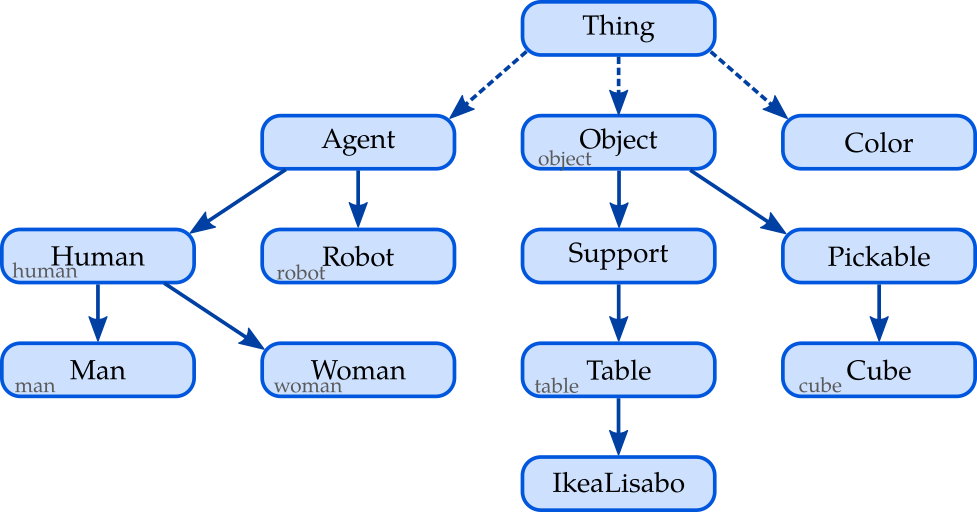
\includegraphics[scale=0.4]{figures/chapter2/Tbox.png}
\caption{\label{fig:Tbox} Representation of an ontology class hierarchy graph to illustrate the composition of a TBox. Taking the class Human, the bottom arrow has to be read as \textit{``A man is a kind of Human''}. The texts at the bottom left of the class, if there is, are the classes' labels in natural language.}
\end{figure}

\improvement{Itemize}
The TBox $\Tbox$ contains assertions about the \textbf{classes} (types) of the ontology. It is defined by $\Tbox = \langle \classset, H \rangle$. It can be seen as a directed acyclic graph as presented in Figure~\ref{fig:Tbox}. $\classset$ is the set of all the classes of the ontology. In our example, $\classset = \{Thing,\ Agent,\ Object, ...,\ IkeaLisabo\}$. Considering the TBox as a graph, $H$ stores its directed edges. They represent the inheritance links between the classes (i.e. the subsumption assertions). We often use the special property ``isA'' to refer to these links (e.g. \textit{(Human, isA, Agent)}). In the OWL language, they are described with the property rdfs:subClassOf, as illustrated in the Listing~\ref{lst:Tbox}.

\noindent
\begin{minipage}{\textwidth}
\begin{lstlisting}[frame=single, basicstyle=\scriptsize\ttfamily, label={lst:Tbox}, caption={Description of ontology classes in the OWL language using the Turle syntax.},captionpos=b, style=OwlTurtle]
:Human rdf:type owl:Class ;
       rdfs:subClassOf :Agent .

:Man   rdf:type owl:Class ;
       rdfs:subClassOf :Human .
\end{lstlisting}
\end{minipage}

\subsubsection{The ontology RBox: Relations between Roles}

\begin{figure}[ht!]
\centering
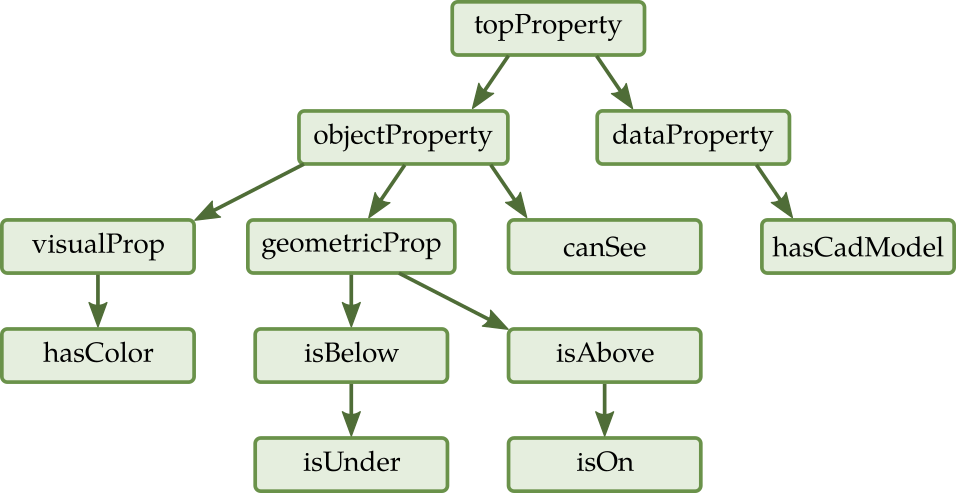
\includegraphics[scale=0.4]{figures/chapter2/Rbox.png}
\caption{\label{fig:Rbox} Representation of an ontology property hierarchy graph to illustrate the composition of an RBox. Taking the property isBelow, the bottom arrow has to be read as: \textit{``The property isUnder is a specification of the property isBelow''}.}
\end{figure}

The RBox $\Rbox$ contains axioms about the \textbf{properties} (roles). It is at least defined by $\Rbox = \langle \propset, \inclset, \invset, \domainset, \rangeset \rangle$. In the same way as the TBox, $\propset$ is the set of properties, and $\inclset$ stores the directed edges of the finite directed acyclic graph representing the inheritance links between the properties. Such a graph is represented in Figure~\ref{fig:Rbox}. These inheritance links aim at specifying properties. In our example, the property IsOn is a specification of the property isAbove in the way that an object being on another is an object that is above the latter and being in contact with. It is described with the property rdfs:subPropertyOf in the OWL language. 
$\invset = \{(\property, \property^{-1}) \in \propset^2\}$ is the set representing the properties inverses (\textit{e.g.} $(isOn, isUnder) \in Inv$). Describing the inverse of a property is useful first to reduce description work since if some describe a relation involving a property for which an inverse is defined, the inverse relation is also described in an underlying way. Moreover, for an algorithm exploring an ontology, knowing that a relation uses a property having an inverse can allow reducing the algorithm complexity by not considering the inverse relation into the exploration.
Finally, $\domainset$ and $\rangeset$ are two sets representing respectively the properties domains and ranges. Their are define by $\domainset = \{(\property, \class)\}$ and $\rangeset = \{(\property, \class)\}$ with $\property \in \propset$ a property and $\class \in \classset$ a class. The domain of a property informs on the type of resources that may use the property, thus the type of the subject of a triplet. The range of a property informs on the valid values applied to the property, thus the type of the object of a triplet. For the property isOn, we would therefore have $(isOn,\ Object) \in \domainset$ and $(isOn,\ Support) \in \rangeset$. In this way, we state that the property IsOn can be used to describe that an object is on top of an object being support. Domains and ranges can be used in two ways. It can be to check the consistency of an ontology by checking if the way the properties have been used corresponds to their definition. It can also be used to reason on the ontology and extract new knowledge from a given situation. If, for example, an entity is said to be on top of another that is not described as being a support, we could deduce that this second entity may be a support.

The formalization above considers only a general kind of property while the OWL language makes the distinction between two main categories. The \textbf{object properties}, linking two entities, and \textbf{data properties}, linking an entity to a value. While both are slightly different, we will only keep a general definition of a property for our formalization to simplify the future algorithm explanations. An example of the description of an object property and a data property from the Figure~\ref{fig:Rbox} are illustrated in the Listing~\ref{lst:Rbox} using the OWL language.

\begin{lstlisting}[frame=single, basicstyle=\scriptsize\ttfamily, label={lst:Rbox}, caption={Description of ontology properties in the OWL language using the Turle syntax.},captionpos=b, style=OwlTurtle]
:isOn  rdf:type owl:ObjectProperty ;
       rdfs:subPropertyOf :isAbove ;
       owl:inverseOf :isUnder ;
       rdfs:domain :Object ;
       rdfs:range :Support .

:hasCadModel rdf:type owl:DatatypeProperty ;
             rdfs:domain :Object .
\end{lstlisting}

\subsubsection{The ontology ABox: Asserting facts}

\begin{figure}[ht!]
\centering
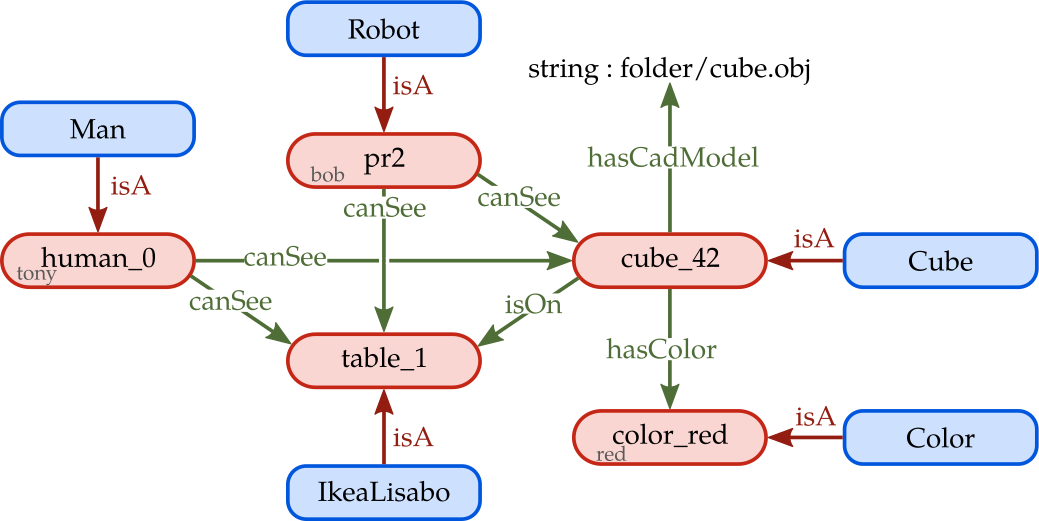
\includegraphics[scale=0.4]{figures/chapter2/Abox.png}
\caption{\label{fig:Abox}  Representation of an ontology instances graph to illustrate the composition of an ABox. Red boxes are individuals of the ontology. Green arrows are properties coming from the RBox and applied to individuals. Red arrows represent a direct inheritance link between an individual and a class coming from the TBox. The texts at the bottom left of the individuals, if there is, are the individuals' labels in natural language.}
\end{figure}

The ABox $\Abox$ contains assertions about the \textbf{entities} (individuals) of the ontology. When we refer about entities, we no more speak about general concepts but rather of instantiated concept, being either a physic or virtual entity. The ABox is defined by $\Abox = \langle \indivset, \inheritset_0, \relationset \rangle$. $\indivset$ is the set of all the entities represented in the ontology. $\inheritset_0$ the set of direct types of $\indivset$ such as $\inheritset_0 = \{(\indiv, \class) \}$ with $\indiv \in \indivset$ an individual and $\class \in \classset$ a class. In the graphical representation of an ABox in the Figure.~\ref{fig:Abox}, the red blocks are the ABox entities ($\indivset = \{human_0,\ pr2,\ ...,\ table\_1\}$) and the red arrows with the label ``isA'' are the intities direct types ($(cube\_42, Cube) \in \inheritset_0$).
$\relationset$ is finally the set of \textbf{relations} between entities. Such relation are in the form of triplets $(\subject, \property ,\object)$ where $\subject$ is the subject, $\property$ the property and $\object$ the object. The set of relations is thus defined by $\relationset = \{(\subject, \property ,\object) | (\subject, \object) \in \indivset^2, \property \in \propset\}$. These relations are represented by the green arrows between the entities in Figure~\ref{fig:Abox}. We can note in this figure the presence of the use of a data property ``hasCadModel''. This property does not link two entities, which goes against the previous definition. Regarding our formalization and to keep it tractable, we can however keep it as it is, and view the string value as an entity having for direct type a concept ``String''. An example of the description of an entity from the Figure~\ref{fig:Abox} is illustrated in the Listing~\ref{lst:Abox} using the OWL language.

\begin{lstlisting}[frame=single, basicstyle=\scriptsize\ttfamily, label={lst:Abox}, caption={Description of an ontology individual in the OWL language using the Turle syntax.},captionpos=b, style=OwlTurtle_indiv]
:cube_42  rdf:type     :Cube ;
          :hasColor    :color_red ;
          :hasCadModel ``folder/cube.obj''^^string ;
          :isOn        :table_1 .
\end{lstlisting}

We just saw that in the ABox, $\inheritset_0$ contains the direct types of entities. We also saw that the classes can inherit from one each other in the TBox, thanks to the classes inheritance directed edges stored in $H$. This means that the individuals of the ABox have inherited types. Taking the entity cube\_42 of Figure.~\ref{fig:Abox}, its direct type is the class Cube ($(cube\_42,\ Cube) \in \inheritset_0$). Regarding the TBox represented in Figure.~\ref{fig:Tbox}, a Cube is a kind of Pickable ($(Cube,\ Pickable) \in H$), itself being a kind of Object ($(Pickable,\ Object) \in H$). We can thus say that the entity cube\_42 is a Cube, a Pickable, and an Object. To represent it, we use $\inheritset$ to denote the set of direct and inherited types. We thus have $\{ (cube\_42,\ Cube), (cube\_42,\ Pickable), (cube\_42,\ Object)\} \subset \inheritset$.

\subsubsection{Extending the ontology TBox}

With the use of the relation set $\relationset$ of the ABox we saw that we can apply properties to individuals to link them together and form relations in the form of triplets. However, some could want to apply properties to classes to describe general links between classes. While properties domains and ranges already give such relations this can be not enough. Taking an object property hasMother, we can assign to it the class Human for domain and Woman for range. With such description, we state that a human CAN have a mother that is a woman but we do not describe that even if we do not know how it is, a human has a mother how is a woman. For this particular example, we could use cardinality constraint but we will not go as far. Taking now the data property hasCadModel of Figure~\ref{fig:Rbox}, we have applied it to a specific entity in the example of Figure~\ref{fig:Abox}. But what about a Table Lisabo (IkeaLisabo in Figure~\ref{fig:Tbox})? Any table of this model will have the same CAD model and we do not want to put this relation to every entity of this type of table. Here domains and range are not sufficient to represent it. To do so, we will use \textbf{annotation properties} applied to classes. Annotation properties are usually used to document ontologies and not to describe general relations on classes. We take thus some liberty regarding the OWL standard for convenience. However, we will try to use it in very particular cases where no other simple solution can be applied. Relations to classes using annotation properties are thus added to the definition of a TBox $\Tbox = \langle \classset, H, \annotationset \rangle$, where $\annotationset$ is the set of relation between classes in the form of triplets.

\subsubsection{Advanced use of properties}

In this sub-section, we present a formalism of an ontology in the form of $\kbs = \langle \Abox, \Tbox, \Rbox \rangle$. All the knowledge stored in $\kbs$ are sufficient to build exploration algorithm on top of it. However, to reason on ontology aditional descriptions are necessary in the form of properties characteristics. We do not add them to the knowledge base formalism but enumerate them bellow: 

\begin{itemize}
	\item \textbf{Symmetric property}: If the relation $(x, p, y)$ holds in $\relationset$ with $p$ being a symmetric property, the relation $(y, p, p)$ is also part of $\relationset$. \\ $hasSpouse$
	
	\item \textbf{Asymmetric property}: If the relation $(x, p, y)$ holds in $\relationset$ with $p$ being an asymmetric property, the relation $(y, p, p)$ can no be part of $\relationset$. \\ $hasChild$
	
	\item \textbf{Reflexive property}: A reflexive property can be used to link an individual to itself. \\ $hasRelative$
	
	\item \textbf{Irreflexive property}: An irreflexive property can not be used to link an individual to itself. \\ $hasParent$
	
	\item \textbf{Functional property}: Every individual can be linked by a functional property to at most one other individual. By this way, if ${(x, p, y), (x, p, z)} \subset \relationset$, then $y = z$. \\ $hasFather$
	
	\item \textbf{Inverse functional property}: Every individual can holds an iverse functional property at most one. By this way, if ${(x, p, y), (z, p, y)} \subset \relationset$, then $x = z$. \\ $hasHusband$
	
	\item \textbf{Transitive property}: A transitive property describe a link between two individuals x and z whenever it exist a link between x and y, and y with z with this property. If ${(x, p, y), (y, p, z)} \subset \relationset$ with p a transitive property, then $(x, p, z) \in \relationset$. \\ $hasAncestor$
	
	\item \textbf{Property chain axiom}: While the transitive property characteristic decsribe a link between several individuls with the same property, the chain axiom does the same with distinct properties. Given the chain $p_1 \bullet p_2 \Rightarrow p_3$, if ${(x, p_1, y), (y, p_2, z)} \subset \relationset$, then $(x, p_3, z) \in \relationset$. \\ $hasParent \bullet hasParent \Rightarrow hasGrandparent$
	
	\item \textbf{Disjunction}: Given two disjoint elements (classes or properties), a third element can not inherit of the both disjoint elements. \\ $Man \sqcup Woman$
\end{itemize}

\subsubsection{Labeling functions}

We saw in the previous chapter that the semantic knowledge base is part of what we assimilate to be the declarative memory. The particularity of such memory is the ability to speak about the knowledge it stores. In this way, we introduce a labeling function $\labelfunc$ for any element of the ontology. This labeling function is specified for the individuals ($\alabel$), the classes ($\tlabel$), and the properties ($\plabel$). Considering the individuals labeling function $\alabel: \indivset \rightarrow Lbl$ with $Lbl$ a set of communicable names encoded as UTF8 string in our implementation. The same holds for the other two labeling functions.

\subsubsection{Ontology for Human-Robot Interaction}

Because we are working in the field of Human-Robot Interaction, it is mandatory for the robotic agent to be able to represent its own knowledge but also to represent an estimate of its human partners' knowledge. Such features will be explained later in this thesis and we only introduce the related notation for the moment.
We define the robot's own simbolic knowledge base $\kbs^R = \langle \Abox^R, \Tbox^R, \Rbox^R\rangle$.
Then, for each human agent $H_i$ the robot knows, we concider the agent's semantic knowledge $\kbs^{H_i} = \langle \Abox^{H_i}, \Tbox^{H_i}, \Rbox^{H_i} \rangle$.
The robot's global knowledge thus encompasses both its own semantic representation of the environment as well as an \textbf{estimation} of the other agent's knowledge.
In the rest of this thesis, we will simply use the notation $\kbs$ in cases where the used knowledge base does not matter.

\subsubsection{Ontology formalism recap}

The ontology definition used all along this thesis is summarized in Table~\ref{tab:onto_symboles}.

\begin{table}[ht!]
\caption{The list of symbols of used to define a semantic knowledge base as an ontology }
\label{tab:onto_symboles}
\begin{tabular}{ll}
{\ul \textbf{$\Abox$ ABox entities/indiv}} & {\ul \textbf{$\Tbox$ TBox classes/concepts}}  \\
$\indivset$: set of entities               & $\classset$: set of classes  \\
$\inheritset_0$: entities' direct types        & $H$: classes inheritance links \\
$\relationset$: relations between entities    & $\annotationset$: relations between classes  \\
$\alabel$: individuals labeling function & $\tlabel$: classes labeling function \\
 & \\
\multicolumn{2}{l}{{\ul \textbf{$\Rbox$ RBox roles/properties}}}                          \\
$\propset$: set of properties              &                                              \\
$\inclset$: properties inheritance links       & $\invset$: properties inverses                   \\
$\domainset$: properties' domains sets     & $\rangeset$: properties' ranges sets   \\
$\plabel$: properties labeling function & \\
\end{tabular}
\end{table}

\section{Architecture}

\subsection{Permanent versus temporary data structure}

\subsection{Concepts' identifier versus name in natural language}

\subsection{Resoning to enrich the knowledge}



\section{Managing others' estimated knowledge}

\subsection{Ontologenius multi-instances principle}

\subsection{Catching knowledge at a given moment}

\subsection{Exploring several possible mental states at once}



\section{Using Ontologenius in robotic applications}

\subsection{Inserting new knowledge}

\subsection{Retrieving knowledge}

\subsubsection{Low-level queries}

\subsubsection{SPARQL-like queries}

\subsection{Interfacing with Ontologenius}

To work with Ontologenius in the easiest way as possible, we provide to the users several tools. Here we present the Application Programming Interface (API) and the debugging Graphical User Interface (GUI).

\subsubsection{The Application Programming Interfaces}

To provide an abstraction of the ROS middleware, and thus of the ROS messages, we propose two API to use Ontologenius. One is in C++\footnote{\url{https://sarthou.github.io/ontologenius/cpp_API/CppAPI.html}} and the other in Python\footnote{\url{https://sarthou.github.io/ontologenius/python_API/PythonAPI.html}}. Both are constructed in the same way and use approximately the same methods names to easily go from one to the other depending on the needs. They are composed of 13 classes for a total of more than 90 distinct methods. Such a number of methods allow a fine and precise use that it is for the instance management, the reasoners' management, the knowledge insertion, or the ontology query. In addition, the methods support all the exploration options in an intuitive way.

The API also take advantage of advanced ROS use for the services. It provides a direct TCP connection with a recovery mechanism. For intensive query use in a limited time, the first query will take more time to establish a direct connexion and all the following will benefit from it. It thus provides efficient and safe communication without additional complexity for the users.

Finally, to take Ontologenius in hand and its APIs, Ontologenius comes with five tutorials\footnote{\url{https://sarthou.github.io/ontologenius/cpp_Tutorials/Tutorials.html} and \url{https://sarthou.github.io/ontologenius/python_Tutorials/Tutorials.html}} covering its more basic usage to the more complex ones including the use of the versioning mechanism.

All the APIs description and the tutorials are available online on a website dedicated to Ontologenius: \url{https://sarthou.github.io/ontologenius}.

\subsubsection{Debbuging tool}

To help new users to take in hand Ontologenius and to help more experienced users to debug their applications using Ontoloegnius, we provide a Graphical User Interface (GUI). It has been developed using Qt which allows easy development of GUI. It is linked to ROS and provides almost all the methods available with the API like the instance management, the reasoners' management, the knowledge insertion, and the ontology query. In addition, for all the exploration queries, hovering a button provides a brief explanation of the hovered method and its equivalent in the ROS command lines.

\begin{figure}[ht!]
\centering
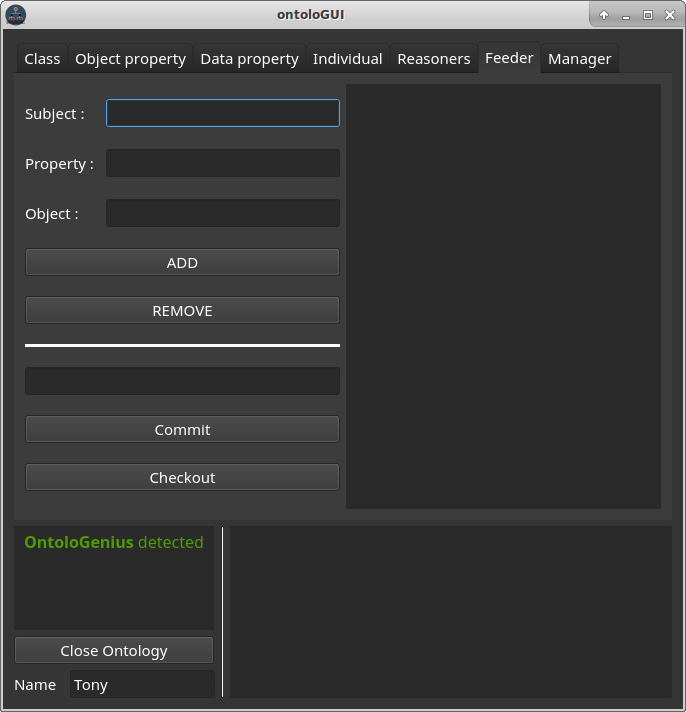
\includegraphics[scale=0.5]{figures/chapter2/ontologui.png}
\caption{\label{fig:chap2_ontologui} A view of the Ontologenius Graphical User Interface. With the displayed panel a user can insert or remove triplets from a given instance. On the left-hand bottom, we can see that the current instance is called Tony.}
\end{figure}

During this chapter, we saw that Ontologenius is base on a lot of low queries for a precise and efficient exploration of an ontology. This GUI is thus often used during the development of an application using Ontologenius to choose the right method to use by allowing the developer to directly test the kind of result he can expect with a given query. In addition, at run-time developers can easily explore the \acrshort{kb} to understand the origin of bugs in their application.

\section{Computational preformance evaluation}

In this section, we evaluate the Ontologenius performance and scalability through comparison with two systems and using their own tests. First, we compare with the KnowRob system with a focus on required CPU time to insert new knowledge and required memory to store this knowledge. The second system of comparison is ORO. With this latter, we measure query resolution time. Finally, we present some additional measures like concept recovery time and \sparql{} query resolution time.

\subsection{Comparing with Knowrob}

We start these comparisons with the KnowRob system presented in~\cite{tenorth_2013_knowrob}. This system is composed of several modules able to perform dedicated reasoning like temporal reasoning, CAD model segmentation, or object perception. All these modules are integrated around the logical programming language SWI Prolog~\cite{wielemaker_2012_swi}. OWL ontologies are loaded using the SWI Prolog’s Semantic Web library~\cite{wielemaker_2003_prolog} which provide a performant and scalable way to manipulate RDF structure in Prolog. Internally, the triple structure of the ontologies is represented as Prolog predicates. At the difference of Ontologenius, the Prolog system and thus KnowRob does not aim to be used as a server but rather as a monolithic and highly integrated system. To provide a fair comparison, in the part, we used Ontologenius without the ROS communication layer. Consequently, a single process runs both ontologenius and the test application.

The article~\cite{tenorth_2017_representations} propose a detailed presentation of the internal representation of KnowRob and present some performance and scalability analysis. The following comparisons have to be considered carefully. KnowRob is a wider and more mature system than Ontologenius. It proposes more advanced capability in terms of reasoning and integration. Ontologenius is more focused on \acrshort{hri} applications as presented earlier in this section. In this way, some simplifications that have been done to fit at our best the KnowRob tests may impact the results. The final reason why the following results should be taken with caution is that due to the complexity of the KnoRob system, we did not perform their test on our end. The results for the KnowRob system comes from their paper~\cite{tenorth_2017_representations}. Consequently, in this section, we do not aim at showing that Ontologenius is "better" than KnowRob. We rather want to show that Ontologenius is not out of the scope in terms of performance and scalability regarding a well-established software.

For the tests we have replicated, they use the description of visual perception entities. Such an entity represents the occurrence of the perception of a given object, having a given pose at a given instant. An example of one of these entities is illustrated in listing~\ref{lst:chap2_visual_perception}. The entity $cup\_i$ is the perceived object. The entity $VisualPerception\_i$ is the perception occurrence. It uses an object property to make a link with the perceived object and two data properties to represent the object's pose and the perception time stamp. The first simplification we had to make is the representation of the matrix of position. In Ontologenius, the data types are only represented in a serialized way as no internal manipulation of these types are made. Thanks to the use of Prolog, KnowRob can manipulate such a matrix and perform operations on it. Even if it is not said if they have inverse properties or not, we add one for the \textit{objectActedOn} property in order to know in which perception instance an object has been perceived.

\begin{lstlisting}[frame=single, basicstyle=\scriptsize\ttfamily, label={lst:chap2_visual_perception}, caption={Description of a visual perception entity created in a somparable way as in the Knowrob system. The description is provided in the OWL language using the Turle syntax.},captionpos=b, style=OwlTurtle_indiv]
:cup_i  rdf:type   :Cup ;

:VisualPerception_i  rdf:type         :VisualPerception ;
                     :objectActedOn   :cup_i ;
                     :eventOccursAt   [[1,0,0,2.56], ... ,[0,0,0,1]]^^RotMat ;
                     :startTime       6572^^Time .
\end{lstlisting}

\begin{figure}[ht!]
\centering
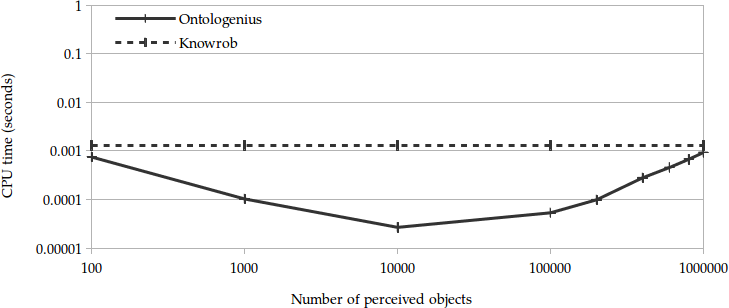
\includegraphics[width=\textwidth]{figures/chapter2/knowrob/Insertion.png}
\caption{\label{fig:chap2_knowrob_insertion} Comparison of the required CPU time for creating large numbers of object perceptions in the knowledge base. Each inserted object correspond to a visual perception entity linked to a cup, a pose matrix, and a time stamp. Ontologenius is used without the ROS communication layer to provide comparable usage and thus results.}
\end{figure}

The first test consists of creating and inserting N visual perception entities in the \acrshort{kb} and measuring the required CPU time to insert one of them Theis means that we measure the average CPU time over N insertions. For each visual perception entity, we thus have to create two entities (the visual perception entity and the perceived object), two inheritance links, two raw data, and three relations (two based on data property and one based on object property). The results are shown in figure~\ref{fig:chap2_knowrob_insertion}. KnowRobs has a constant time around 1.3ms. With Ontologenius we do not have constant time. The first decreasing part can be explained by the asynchronous Ontologenius mechanism. It looks for updates at 20hz. Consequently, we can have a delay between the moment we publish updates and the moment they are processed. The effect of the mechanism disappears with the amount of data to process since once the update mechanism started, it does not stop while data have to be processed. The general trend is thus an increase in the required CPU time. This increase can come from the fact that Ontologenius performs reasoning, like the creation of the inverse relations, at update where KnowRob resolve it at query. In addition, Ontologenius also performs consistency checking at update. However, until 1,000,000 insertions and thus 2,000,000 of entities, 2,000,000 raw data, and 5,000,000 triples (2 for inheritances and 3 for relation per perception entity), the required CPU time is under 1ms.

On the basis of the same insertions as previously, the second test consists of measuring the required memory. The results are shown in figure~\ref{fig:chap2_knowrob_memory}. For a high number of individual, Ontologenius required a bit less memory. It can be explained by the fact that it has a simplified matrix representation. In addition, no information had been provided about the initial content of the~\acrshort{kb}. Both systems, therefore, require memory in the same order of magnitude.

\begin{figure}[ht!]
\centering
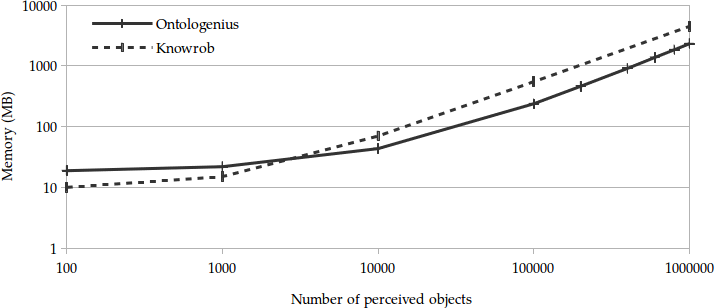
\includegraphics[width=\textwidth]{figures/chapter2/knowrob/Memory.png}
\caption{\label{fig:chap2_knowrob_memory} Comparison of the required memory for creating large numbers of object perceptions in the knowledge base. Each inserted object correspond to a visual perception entity linked to a cup, a pose matrix, and a timestamp. Ontologenius is used without the ROS communication layer to provide comparable usage and thus results.}
\end{figure}

The last test with KnowRob is about the required CPU time to perform queries. They took the same \acrshort{kb} as made previously, with N visual perception entities. The goal here is to select randomly one of the perceived cups, then retrieve its pose. In Prolog, their query is:

\paragraph{?-} owl\_individual\_of(Obj, kr:’Cup’), current\_object\_pose(Obj, Pose).

Using the low-level queries of Ontologenius, we have made a function doing the equivalent. It requests for all the cups, selects one randomly, retrieves the visual perception entity it is linked to, and fetches the pose. The required CPU time is reported in figure~\ref{fig:chap2_knowrob_query}.

\begin{figure}[ht!]
\centering
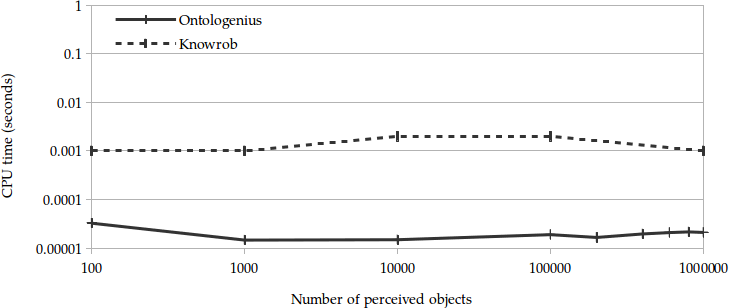
\includegraphics[width=\textwidth]{figures/chapter2/knowrob/Query.png}
\caption{\label{fig:chap2_knowrob_query} Comparison of the required CPU time for querying for the pose matrix of and randomly selected object after that N perception entities have been created. Ontologenius is used without the ROS communication layer to provide comparable usage and thus results.}
\end{figure}

Concerning KnowRob, the query time is almost constant, jumping between one and two milliseconds. It has to be noted that in Prolog, the time measurement resolution is about 1 millisecond. Nevertheless, due to the jump, we can assume that the real value is not far from the millisecond. For Ontologenius, the query time is also almost constant, with values around 0.02ms. This significant difference, with an average factor of 75, can be due to the more precise queries provided by Ontologenius and to the fact that Ontologenius does not have to solve inference at query time. For the more precise queries, submitting a query to Prolog, it has to perform a kind of search among the \acrshort{kb} to make the submitted predicates true. At the difference, Ontologenius requires the programmer to refine and decompose the high-level query, allowing the execution to be more efficient. For the inference, most of the relations are inferred at the update, like the ones coming from inverse properties. At query, Ontologenius only has to go through the existing relations and only reason about the classes and properties inclusion axioms. For example, if we had a query for all the objects, no direct link would have been created between the cups instances and the object class, this part would thus have been solved at query thanks to exploration.

In light of the presented results, even if both software have not the exact same goal, way of use, and maturity, we can at least conclude that Ontologenius is not out of scope with acceptable performance and scalability. Since Ontologenius provide fewer functionalities or at least different ones, the results are encouraging. Having poor results with fewer functionalities would have been more problematic.

\subsection{Comparing with ORO}

For the second comparison, we select the software ORO~\cite{lemaignan_2010_oro}. At the difference of KnowRob which does not address the same applications as our, ORO does. It works as a central server, usable by all the components of architecture and is able to manage several instances at a time. In this way, it has been designed for \acrshort{hri} applications. We can however not three major difference from a technical point of view. It is based on the Jena framework for the RDF triples storage and uses Pellet~\cite{sirin_2007_pellet} for the reasoning part. Pellet supports OWL-DL expressiveness level to perform reasoning where with Ontologenius we are still at the OWL-lite expressiveness. Regarding the way to query the ontology, ORO uses the Jena \sparql{} interface. It also provides some inbuild high-level query made for specific applications. Finally, to communicate with the server, ORO uses a TCP connection with a Telnet protocol.

In the same paper~\cite{lemaignan_2010_oro} they propose three test queries to assess the software performance. We thus reproduce these tests and we add a second dimension being the scalability. Consequently, the three test queries have been performed on \acrshort{kb} of different sizes. Before presenting the results, let us see the content of the test ontology. This ontology does not aim to be semantically correct. We first have three object properties: \textit{isAt}, \textit{isOn}, and \textit{isUnder}. The property \textit{isUnder} is described as being the inverse of \textit{isOn} and \textit{isOn} as being a sub-property of \textit{isAt}. Moreover, the property \textit{isOn} has for domain the class \textit{animal}\footnote{We said that the ontology does not have any real meaning.}. No additional information about this ontology is needed for the presented results.

Before performing any query, N triples are inserted in the \acrshort{kb}. These triples are of the form:

\begin{quote} 
\centering 
individual\_i isOn apple
\end{quote}

In this triple, \textit{apple} is an entity already existing in the ontology and which have as type the class \textit{Plant}. Since the property \textit{isOn} has for domain the class \textit{animal}, all the \textit{individual\_i} should be inferred as inheriting of this latter class. Moreover, because of the inverse property, the inverse relation \textit{(apple isUnder individual\_i)} should exist.

The first test query concerns inheritance. The goal is to retrieve all the individuals inheriting the class \textit{animal}. Regarding the inserted relations, if N relations have been inserted, the query should return the N individuals consequently created, meaning the N \textit{individual\_i}. In \sparql{} the query would be:

\begin{quote} 
\centering 
?i rdf:type animal
\end{quote}

\begin{figure}[ht!]
\centering
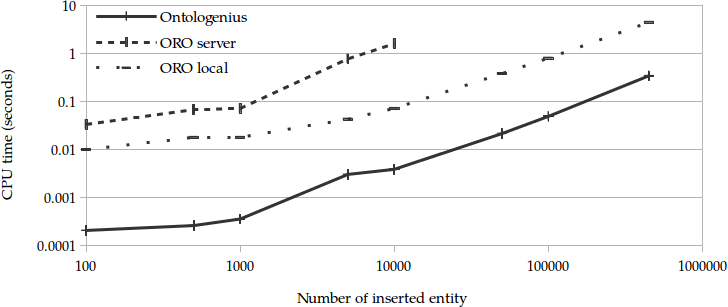
\includegraphics[width=\textwidth]{figures/chapter2/oro/R1.png}
\caption{\label{fig:chap2_oro_r1}Comparison of the required CPU time for querying for all the entities being animal, after that N entity have been created. Ontologenius and ORO are used with their communication layer. To assess the impact of the communication layer on ORO performance, we also provide measures without the ORO communication layer (ORO local).}
\end{figure}

For the test, ORO has been queried through the \sparql{} query where Ontologenius has been queried through low-level queries. To provide results representing the way the software should be used, both have been queried through their respective API. This means that results include the communication times. However, to not fall in a comparison of the communication layers but rather of the software, we have also tested to query ORO without the communication layer. The three plots (one for Ontologenius with the communication layer and two for ORO one with the communication layer and one without) are presented in figure~\ref{fig:chap2_oro_r1}.

First of all, we can note that with the communication layer we have not achieved to go over 10,000 entity with ORO. Rather than a limitation of the software itself, here it is a limitation of the test which require the retrieve of too many entities. Nevertheless, without the communication layer, we succeed to go to 450,000 entities. We can see that Onotlogenius performs far better than ORO, even when ORO is tested without its communication layer. This means that even if the communication time impacts the results, it does not spoil it. In server usage, Ontologenius is more performant of a factor around 255 on average. In this test Ontologenius take advantage of its reasoning process applied at the update, allowing a more direct search.

For the two next queries, we only present the results in server usage as we just saw that this additional time is not inordinate. The second query uses the inverse properties. It aims at retrieving all the entities being under the \textit{apple}. As for the previous query, we thus expect to retrieve the N newly created entities. The corresponding \sparql query is:

\begin{quote} 
\centering 
?i isUnder apple
\end{quote}

The third query is more complex and use a conjunction. The query aims at retreiving all the entity having a relation involving the property \textit{isAt} toward an entity being of type \textit{Plant}. Since all the newly created entities have a relation using the property \textit{isOn}, which is a sub-property if \textit{isAt}, toward the entity \textit{apple}, which inherite of the \textit{Plant} class, the N individual are expected to be retreive. The corresponding \sparql{} query is:

\begin{quote} 
\centering 
?i isAt ?p, ?p rdf:type Plant
\end{quote}

The results of these two queries are presented for both software in figures~\ref{fig:chap2_oro_r3} and~\ref{fig:chap2_oro_r2}. They are appreciably the same as those of the first test query. Ontologenius performs on average better of a factor around 250 and we previously saw that the ORO communication layer has a limited impact which cannot explain such difference.

\begin{figure}[ht!]
\centering
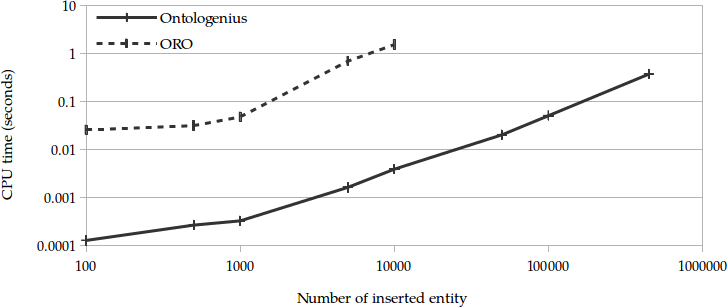
\includegraphics[width=\textwidth]{figures/chapter2/oro/R3.png}
\caption{\label{fig:chap2_oro_r3} Comparison of the required CPU time for querying for all the entities having a relation of the king "isUnder" toward a given entity. Since the invert relation has been inserted for all the created entity, the software have to solve the inverse relation to answer the query. Ontologenius and ORO are used with their communication layer.}
\end{figure}

\begin{figure}[ht!]
\centering
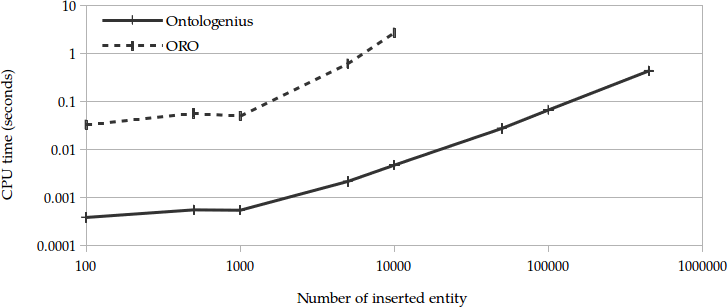
\includegraphics[width=\textwidth]{figures/chapter2/oro/R2.png}
\caption{\label{fig:chap2_oro_r2} Comparison of the required CPU time for querying for all the entities having a realtion of the king "isAt" toward an entity of type "Plant". Ontologenius and ORO are used with their communication layer.}
\end{figure}

Through the comparison with ORO, considering its expected usage, we can fairly conclude that Ontologenius seems to be more adapted for performance requirement. Nevertheless, the test itself could be discussed. The fact that the software have to retrieve such an amount of entity does not represent real use-cases. Moreover, in the light of such equivalent results from a query to another, we can question what is really measured here. Looking backwards to the tests with KnowRob, the query time of Ontologenius was quite constant where here we have a constant increase. This test is however complementary with the ones of KnowRob, showing its ability to retrieve a large number of entities. In addition, even with few entities (100), the performance gap is still significant, confirming the usability of Ontologenius even if it is not based on any more or less established library like Jena or Pellet. 

\subsection{Additional tests}

With the previous tests, we have performed comparisons based on tests proposed by others contributions. We now present some additional tests to assess the performance of Ontologenius. Among the number of features, we have selected two of them to asses.

We first propose to compare the required CPU time to retrieve an entity by its name in natural language and its identifier. For this test, we have taken 466,508 English words. These words have a length going from 1 letter to 45 letters with a means of  9.42 words. For each step of the test, N words have been randomly selected and inserted in the ontology as individuals. In addition, to each entity, we have defined a name in natural language, which is the same as the identifier. The N inserted entities have then been retrieve with their name in natural language and their identifier. The results are presented in figure~\ref{fig:chap2_extra_find}. The retrieve of an entity through the use of its identifier is constant with a required CPU time of around 0.046ms. At the difference, retrieving an entity through the use of its name in natural language is highly impacted by the size of the \acrshort{kb}. We reach a CPU time of 0.62ms for a \acrshort{kb} with 450,000 entity. This result highlights the fact that the name in natural language should be used, with Ontologenius, as an interface with the human partner and that all the algorithm should rather use the identifier. Even if this result could seem evident, it still shows the constant CPU time with the use of identifier, and that even with large \acrshort{kb}.

\begin{figure}[ht!]
\centering
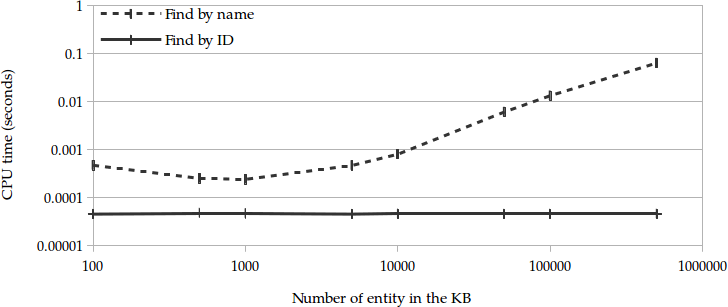
\includegraphics[width=\textwidth]{figures/chapter2/extra_tests/find.png}
\caption{\label{fig:chap2_extra_find} Comparison of the required CPU time to retreive an entity by its name in natural language and its identifier. Ontologenius is used with its communication layer for both cases.}
\end{figure}

The second feature of Ontologenius we choose to evaluate is the instance copy. As explained earlier in this chapter, with Ontologenius we are able to make a deep copy of an ontology instance, resulting in a new and independent instance. Moreover, we have presented a kind of versioning mechanism allowing to represent multiple knowledge state in a single instance. We explained that the expected usage is to perform a single copy to create an independent instance, not altered by other components, then to use the versioning mechanism on the newly created instance. The presented test aims a measuring the required CPU time to perform such a copy, depending on the ontology size.

\begin{figure}[ht!]
\centering
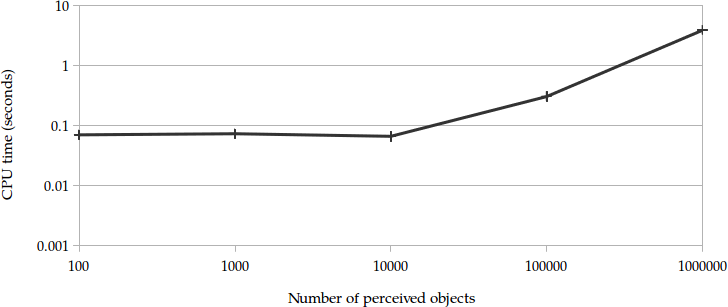
\includegraphics[width=\textwidth]{figures/chapter2/extra_tests/deepcopy.png}
\caption{\label{fig:chap2_extra_deepcopy} Evaluation of the required CPU time to perform a deep-copy depending on the number of perceived entity, represented in the Knowledge Base. Ontologenius is used with its communication layer. }
\end{figure}

For this test, we have taken again, the ontology content proposed by the KnowRob tests. It consists of inserting visual perception structures. We thus add N structures resulting in the creation of 2*N entity, 2*N raw data, 2*N inheritance link, and 3*N relations. Once the N structure inserted, we performed an instance copy and measured the required CPU time. The results for N going from 100 to 1,000,000 are represented in figure~\ref{fig:chap2_extra_deepcopy}. As expected, the required CPU time grow with the \acrshort{kb} size. Starting around 100ms for the smallest \acrshort{kb}, it grew to 4s for the largest one. Even if the results seem acceptable regarding the job to perform, we can however conclude that such an operation should not be performed too frequently. This reinforces the idea of doing a single copy then using the versioning mechanism if we want to represent many states of the same \acrshort{kb}.